% 五号字体,开明式标点处理,不设置默认字体
\documentclass[UTF8,12pt,punct=kaiming,fontset=none]{ctexart}
\usepackage{fontspec}  % 字体
\usepackage{subcaption}  % 节标题
% 品红色链接和注释
% \usepackage[colorlinks=true, linkcolor=magenta, citecolor=magenta, urlcolor=magenta]{hyperref}
% 黑色链接和注释
\usepackage[colorlinks=true, linkcolor=black, citecolor=black, urlcolor=black]{hyperref}
\usepackage{geometry}  % 页面布局
\usepackage{fancyhdr}  % 页眉页脚
\usepackage{titlesec}  % 标题
\usepackage{caption}  % 图表标题
\usepackage{floatrow}  % 图表排版
\usepackage{graphicx}  % 图片路径
\usepackage[pages=some]{background}  % 封面
\usepackage{pdfpages}  % 正文

% 图片路径
\graphicspath{{figures/}}

% 封面
\backgroundsetup{
    scale=1,
    color=black,
    opacity=1,
    angle=0,
    contents={
        \includegraphics[width=\paperwidth,height=\paperheight]{cover.png}
    }
}

% 字体
\setCJKmainfont{Source Han Serif SC}
\setCJKsansfont{Source Han Sans SC}
\setmainfont{CMU Serif}

% 布局
\geometry{a4paper,left=2cm,right=2cm,top=2.5cm,bottom=2.5cm}
\setlength{\headheight}{25pt}

% 页眉页脚
\pagenumbering{arabic}
\pagestyle{fancy}
\fancyhead[L]{· \hspace{0.1cm} \thepage \hspace{0.1cm} ·}
\fancyhead[C]{红石数电评论\\\scriptsize{Review of Redstonic Digital Circuit}}
\fancyhead[R]{第1期\\\scriptsize{2022年2月}}
\fancyfoot[L,C,R]{}


\begin{document}

% 封面
\thispagestyle{empty}
\BgThispage
\quad

% 目次
\newpage
\setcounter{page}{1}
\tableofcontents

% 正文
% \foreach \filename in {
%     基于基本红石电路的函数绘图显示器,
%     基于石墙电路的随机存取存储器,
%     基于石墙控制线的存储器内的微时序特性分析及应用,
%     基于RV32M标准的运算器实现,
%     更高效的乘法器——树状乘法器原理与建造,
%     串行二进制转十进制方案,
%     潜影盒存储——不可堆叠物品解码方案,
%     潜影盒倒序装填器
% }{
%     \includepdf[pages=-]{../预印本/\filename/\filename.pdf}
% }
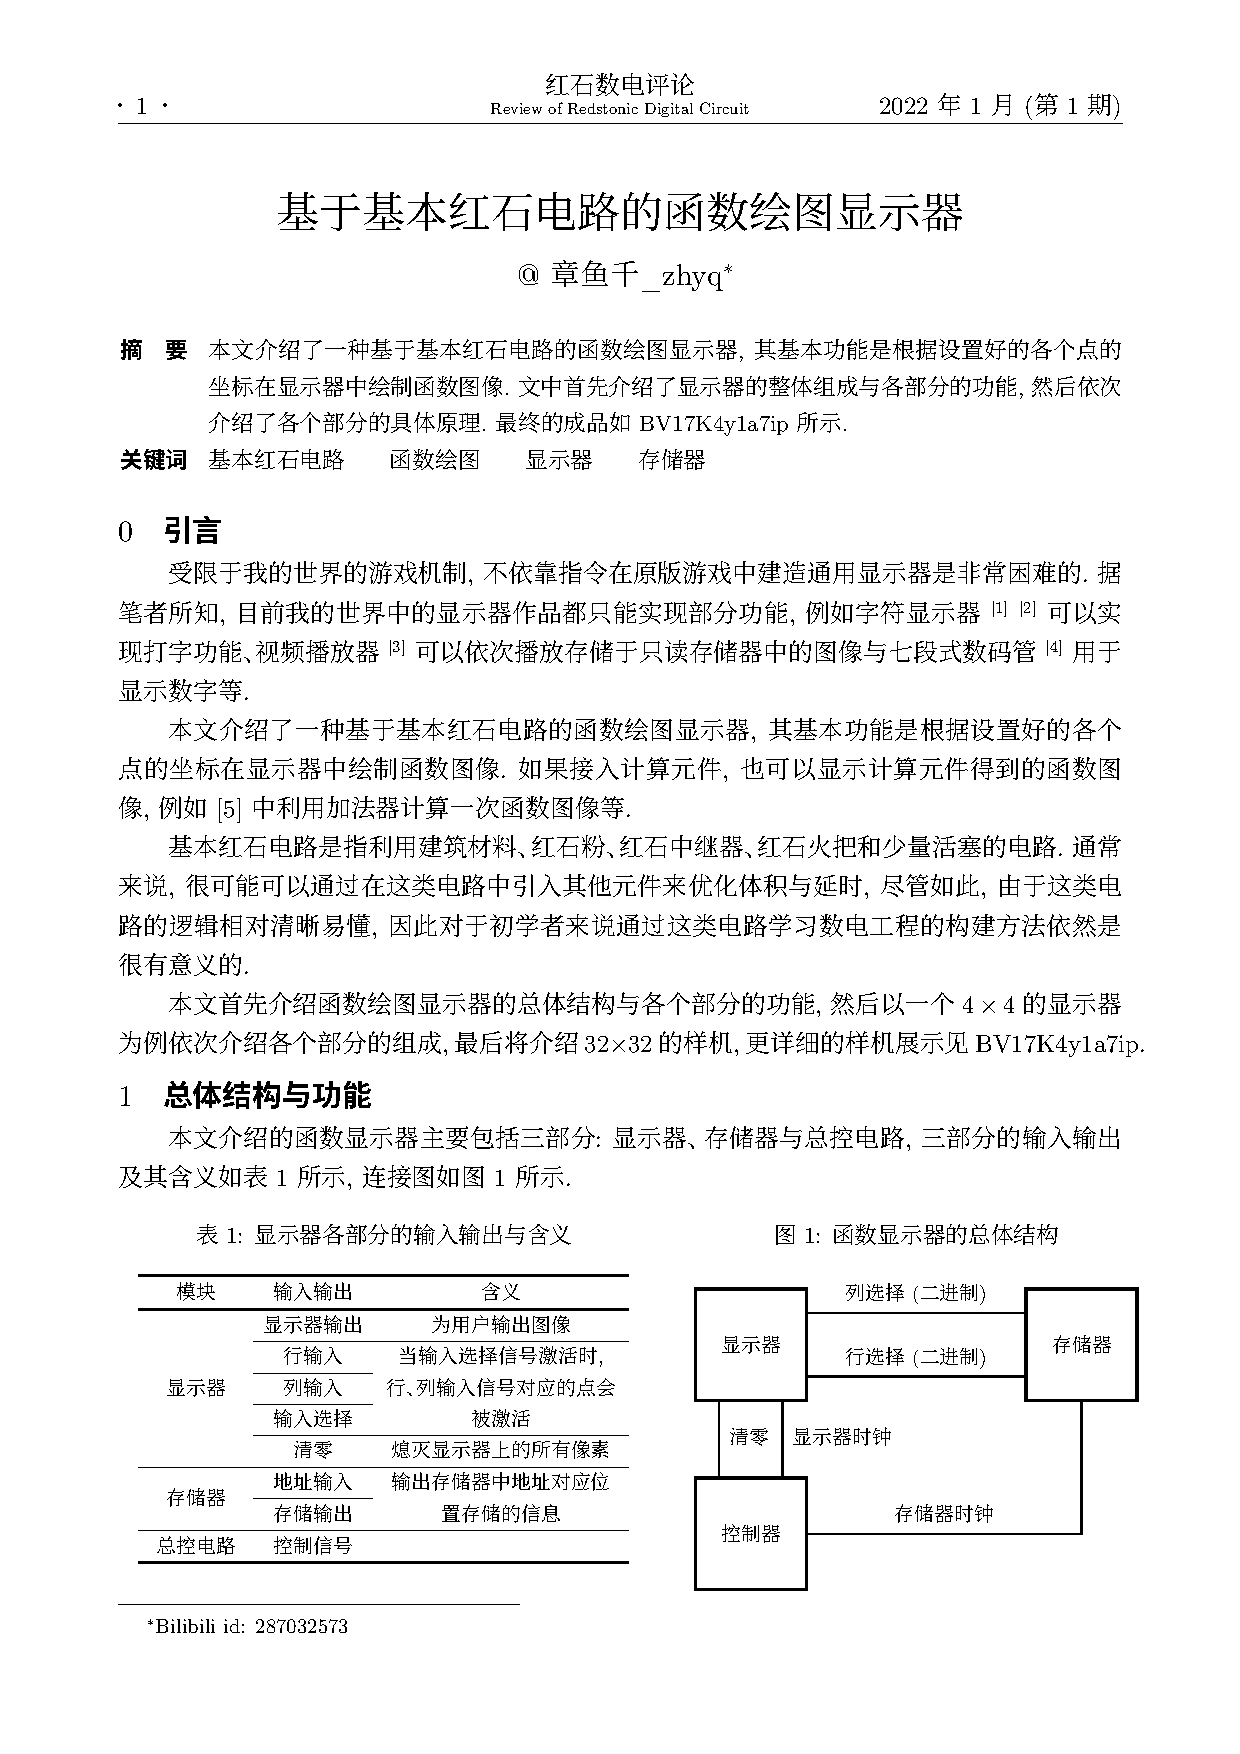
\includepdf[pages=-]{../预印本/基于基本红石电路的函数绘图显示器/基于基本红石电路的函数绘图显示器.pdf}
\includepdf[pages=-]{../预印本/基于石墙电路的随机存取存储器/基于石墙电路的随机存取存储器.pdf}
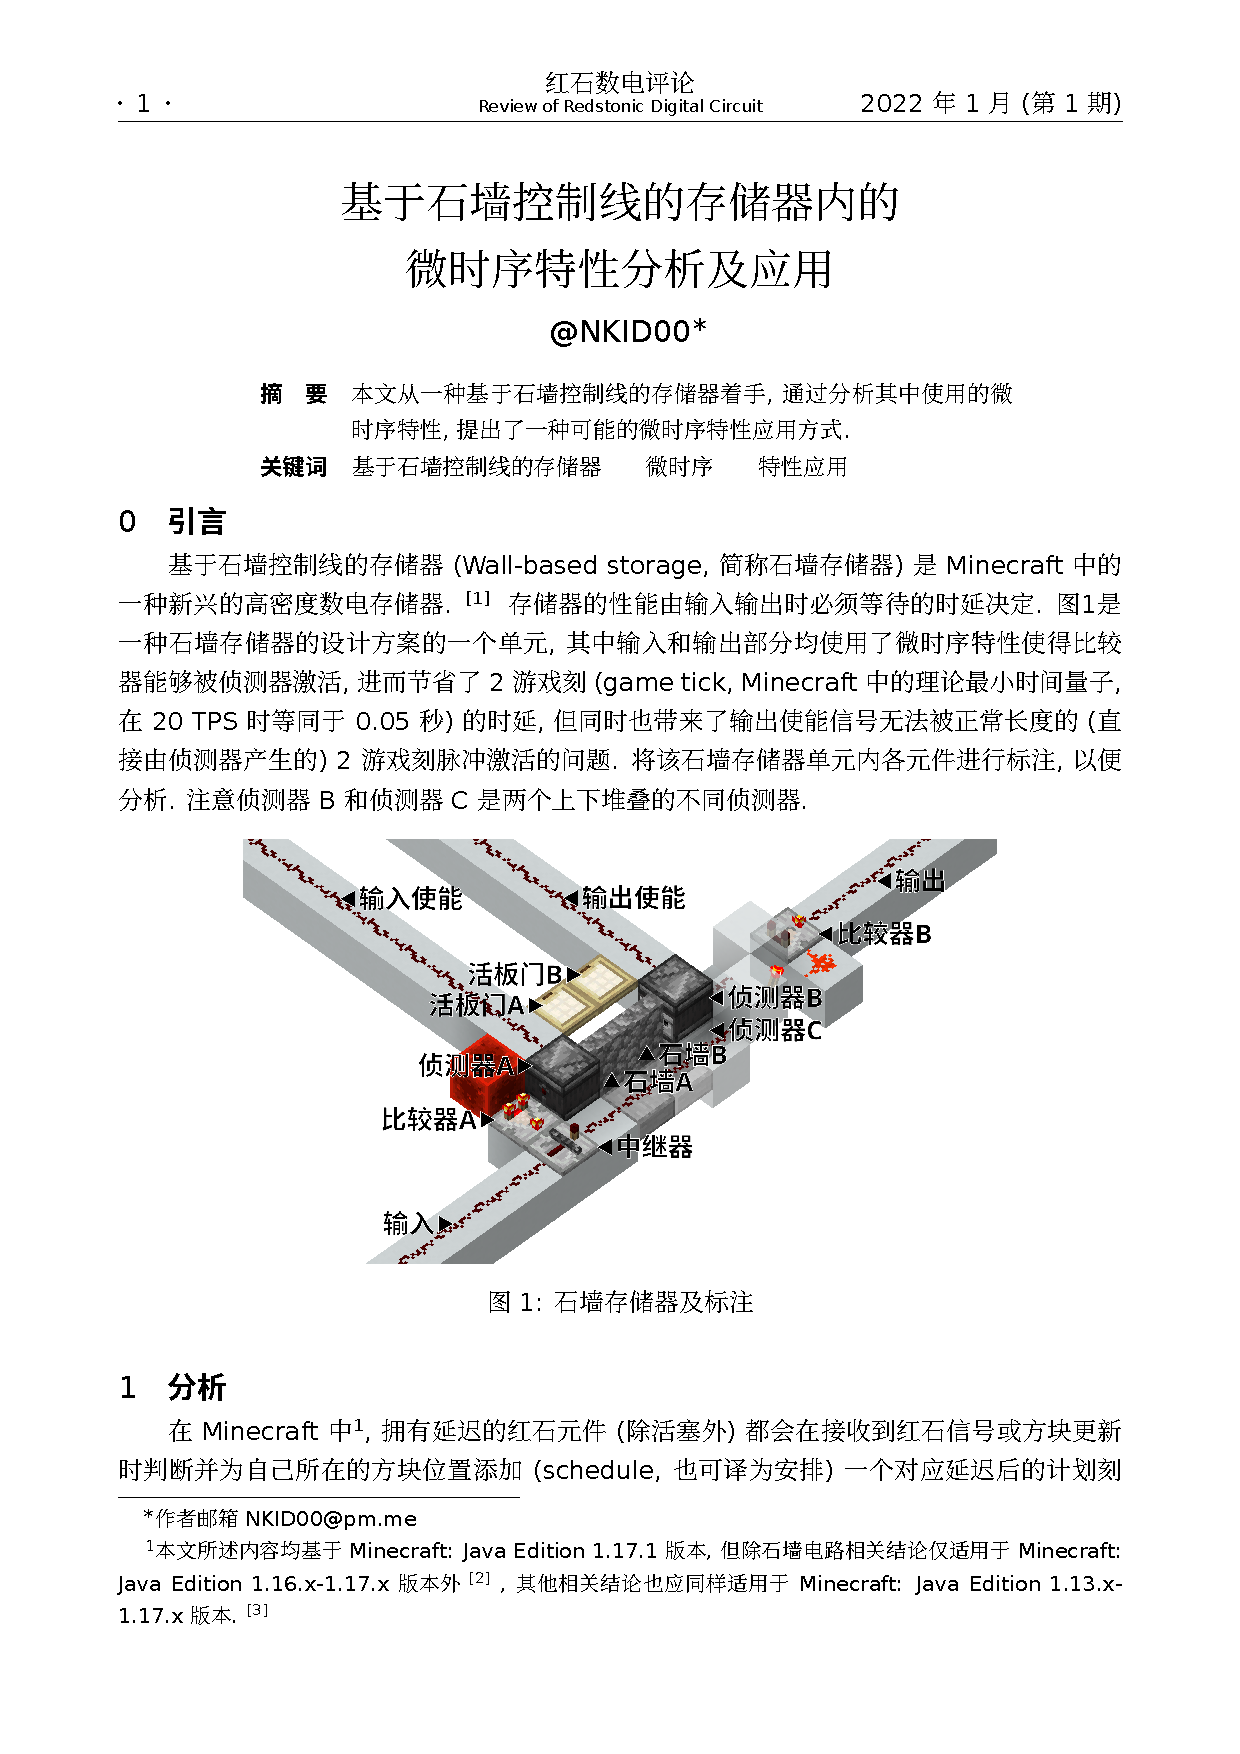
\includepdf[pages=-]{../预印本/基于石墙控制线的存储器内的微时序特性分析及应用/基于石墙控制线的存储器内的微时序特性分析及应用.pdf}
\includepdf[pages=-]{../预印本/基于RV32M标准的运算器实现/基于RV32M标准的运算器实现.pdf}
\includepdf[pages=-]{../预印本/更高效的乘法器——树状乘法器原理与建造/更高效的乘法器——树状乘法器原理与建造.pdf}
\includepdf[pages=-]{../预印本/串行二进制转十进制方案/串行二进制转十进制方案.pdf}
\includepdf[pages=-]{../预印本/潜影盒存储——不可堆叠物品解码方案/潜影盒存储——不可堆叠物品解码方案.pdf}
\includepdf[pages=-]{../预印本/潜影盒倒序装填器/潜影盒倒序装填器.pdf}

\end{document}
